\section{MODELAGEM \textit{BITSTRING} AOS AGENTES}
\label{sec:modelagemBitstring}

A modelagem \textit{bitstring} realizada para a representação do agente é baseada na manipulação direta dos \textit{bits} em uma palavra computacional, que é utilizada para caracterizar sem ambiguidade a especificação do agente $\chi(t)$.

Ao emprego de um modelo em \textit{bitstring} é necessário utilizar uma linguagem de programação com suporte apropriado às operações diretas com \textit{bits}. Desta forma, à implementação do sistema multiagente é empregada a linguagem de programação C++, que provê suporte aos propósitos de modelagem, implementação e paralelização do sistema. 

À representação e armazenamento dos agentes na linguagem de programação escolhida é definida uma estrutura contendo três atributos, em que o primeiro atributo é um inteiro de $16$ \textit{bits} e os outros dois atributos são inteiros de $32$ \textit{bits}. Cada um destes atributos são denominados palavras. Considerando esta estrutura a representação de um agente em memória totaliza $80$ \textit{bits}, que são suficientes ao armazenamento de todos os atributos modelados nesta especificação. 

A manipulação de dados representados em \textit{bitstring} pode utilizar operações lógicas \textit{bit} a \textit{bit} e deslocamentos aritméticos e circulares. Em deslocamentos aritméticos, como aqueles que são definidos na linguagem C++, ocorre a preservação do \textit{bit} de sinal, quando da sua execução no sentido esquerda-direita. Deslocamentos que não preservam o \textit{bit} de sinal são chamados deslocamentos lógicos, que não são definidos na linguagem C++. O uso de tipos de dados \textit{unsigned} descarta a preservação de sinal na realização de deslocamentos, evitando a introdução de erro na manipulação dos \textit{bits} mais significativos em operações de captura e atualização de atributos de um agente, viabilizando o uso de deslocamentos aritméticos com o mesmo resultado prático obtido por deslocamentos lógicos, sendo o uso de tipos \textit{unsigned} em C++ justificado por este motivo. Em deslocamentos circulares, os \textit{bits} que são expelidos de uma extremidade da palavra são inseridos na sua extremidade oposta, preservando-se desta forma os \textit{bits} internos à palavra. Na modelagem considerada não são utilizados deslocamentos circulares. 

Nas próximas sub-seções são apresentadas as modelagens \textit{bitstring} realizadas para os agentes e são descritas as faixas designadas para cada atributo considerado e as operações \textit{bitstring} executadas na captura e atualização dos valores dos atributos dos agentes.

\newpage

\subsection{Modelagem \textit{bitstring} ao Agente}

A modelagem dos agentes é realizada utilizando-se $1$ palavra de $16$ \textit{bits} e $2$ palavras de $32$ \textit{bits}, representadas pelos tipos \textit{uint16\_t} e \textit{uint32\_t} na linguagem C++. Especificou-se ao modelo, que os atributos do agente, descritos em (\ref{eq:especificacaoAgente}) tivessem as designações e representações conforme sintetizadas na Tabela \ref{tab:atributosBitstring}:
\begin{table}[H]
\centering
\begin{tabular}{c|c|c}
 \textbf{Atributo} 			& \textbf{\textit{Bits}}	& \textbf{Valores} 	\\ \hline
 Sexo, $S$ 				& $1$				& $2$	  		\\
 Faixa etária, $FE$ 			& $3$				& $4$	  		\\
 Contador de transições de estados, $C$ & $9$				& $512$	  		\\
 Saúde, $SD$	 			& $3$				& $8$	  		\\ 
 Latitude, $X$ 				& $19$				& $524.288$  		\\
 Lote, $L$				& $13$				& $8.192$  		\\
 Longitude, $Y$ 			& $23$				& $8.388.608$ 		\\
 Quadra, $Q$				& $9$				& $512$	  		\\
 \end{tabular}
\caption{Tabela indicando as quantidades de \textit{bits} e valores distintos possíveis à representação dos atributos do agente $\chi(t)$ modelado.}
\label{tab:atributosBitstring}
\end{table}

A Figura \ref{fig:tiraBitstring} ilustra as três palavras que constituem a tira \textit{bitstring} do agente. A palavra $(1)$ contém os elementos do identificador do sexo $S$ na posição $15$, do identificador da faixa etária $FE$ nas posições $14$ a $12$, do contador de transições de estados $C$ nas posições $11$ a $3$ e do identificador da saúde $SD$ nas posições $2$ a $0$. A palavra $(2)$ armazena os elementos da coordenada $X$ nas posições $31$ a $13$ e do identificador do lote $L$ nas posições $12$ a $0$. A palavra $(3)$ armazena a coordenada $Y$ nas posições $31$ a $9$ e do identificador da quadra $Q$ nas posições $8$ a $1$.

\begin{figure}[H]
 \centering
 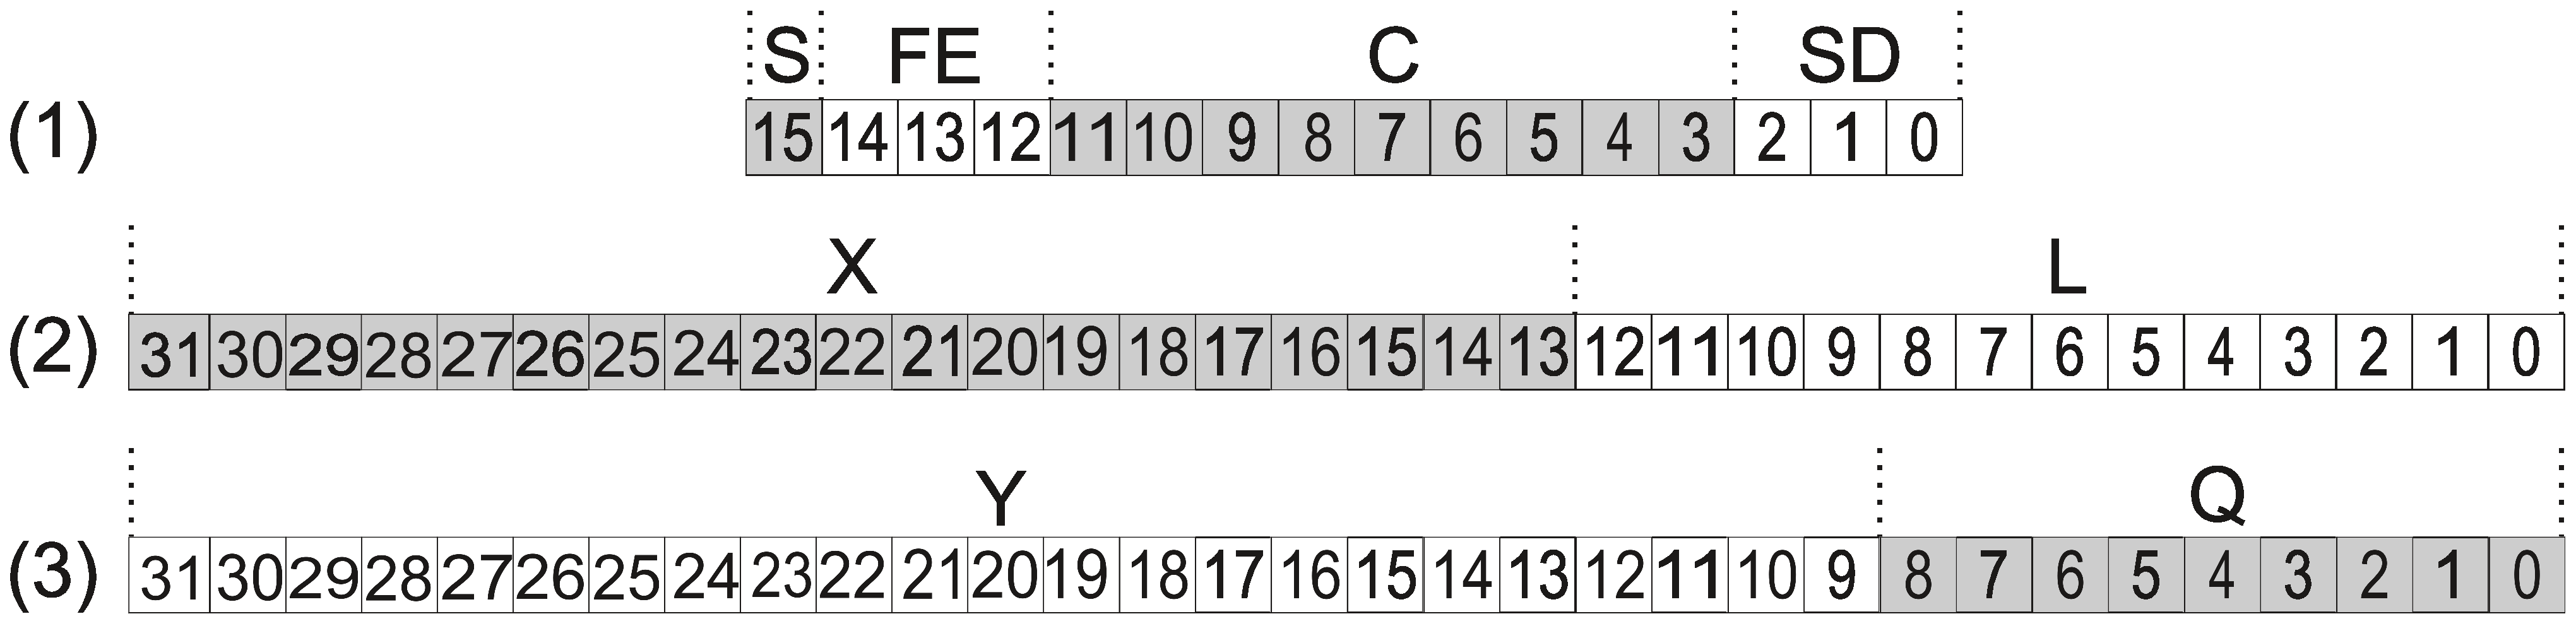
\includegraphics[width=1.0\textwidth]{Figuras/ModelagemBitstring/Tira.eps}
 \caption{Representação \textit{bitstring} do agente $\chi$.}
 \label{fig:tiraBitstring}
\end{figure} 

Considerando as escolhas realizadas à sua modelagem, um agente $\chi$ qualquer do modelo pode ser representado em \textit{bits} como em (\ref{eq:tiraBitstring}), em que os índices subscritos indicam as posições dos \textit{bits} ocupadas pelo atributo e os índices sobrescritos indicam as palavras correspondentes na tira.
\begin{equation}
\begin{split}
 \chi(t)  \equiv  & \big(s_{[15]}; fe_{[14, 12]}, c_{[11, 3]}, sd_{[2, 0]}\big)^1 \\
		  & \big(x_{[31, 13]}; l_{[12, 0]}\big)^2 \\
		  & \big(y_{[31, 9]}; q_{[8, 0]}\big)^3
 \label{eq:tiraBitstring}
\end{split}
\end{equation}

As características que definem o agente $\chi(t)$ devem ser definidas para o ciclo $t$ considerando-se as quantidades de \textit{bits} anteriores à cada atributo e seu tamanho em \textit{bits}. A quantidade de \textit{bits} anteriores a cada atributo é a quantidade de \textit{bits} existentes que são menos significativos que aqueles do atributo em questão. O tamanho em \textit{bits} de um atributo é a quantidade de \textit{bits} utilizada para armazenar as informações pertinentes a tal atributo. Para tomar somente os \textit{bits} necessários às operações, são empregadas máscaras auxiliares à captura dos atributos, utilizando-se deslocamentos não circulares à esquerda e à direita na palavra, na quantidade de \textit{bits} necessária.

Assim sendo, à modelagem dos agentes considera-se que $\# W$ designa o tamanho em \textit{bits} de cada um dos atributos $S$, $FE$, $C$, $SD$, $X$, $L$, $Y$ e $Q$ do agente $\chi(t)$, de modo que se $W \in \left\{S, FE, C, SD, X, L, Y, Q\right\}$, e então a expressão (\ref{eq:tamanhosAtributos}):
\begin{equation}
\# W=
 \begin{cases} 
 1 \quad &se \quad W=S  \\
 3 \quad &se \quad W=FE \\
 9 \quad &se \quad W=C  \\
 3 \quad &se \quad W=SD \\ 

 19 \quad &se \quad W=X \\ 
 13 \quad &se \quad W=L \\
 
 23 \quad &se \quad W=Y \\
 9  \quad &se \quad W=Q \\
 \end{cases}
 \label{eq:tamanhosAtributos}
\end{equation}

Igualmente, à quantidade de \textit{bits} anteriores a cada atributo, $AW$, obtém-se a expressão (\ref{eq:anterioresAtributos}):
\begin{equation}
\# AW=
 \begin{cases}
 15 \quad &se \quad W=S  \\
 12 \quad &se \quad W=FE \\
 3  \quad &se \quad W=C  \\
 0  \quad &se \quad W=SD \\
 
 13 \quad &se \quad W=X  \\
 0  \quad &se \quad W=L  \\
 
 9  \quad &se \quad W=Y  \\
 0  \quad &se \quad W=Q  \\
 \end{cases}
 \label{eq:anterioresAtributos}
\end{equation}

As máscaras empregadas para setar as posições dos elementos que são operados, $MW$, e seus complementos lógicos, $\neg MW$, segundo as especificações às quantidades de \textit{bits} à cada atributo das palavras \textit{bitstring} são especificadas como (\ref{eq:mascarasPositivas}) e (\ref{eq:mascarasNegativas}):
\begin{equation}
 \begin{cases}
 MS  &= 1000000000000000 \\
 MFE &= 0111000000000000 \\
 MC  &= 0000111111111000 \\
 MSD &= 0000000000000111 \\
 
 MX  &= 11111111111111111110000000000000  \\
 ML  &= 00000000000000000001111111111111  \\
 
 MY  &= 11111111111111111111111000000000  \\
 MQ  &= 00000000000000000000000111111111  \\
 \end{cases}
 \label{eq:mascarasPositivas}
\end{equation}

\begin{equation}
 \begin{cases}
 \neg MS  &= 0111111111111111 \\
 \neg MFE &= 1000111111111111 \\
 \neg MC  &= 1111000000000111 \\
 \neg MSD &= 1111111111111000 \\
 
 \neg MX  &= 00000000000000000001111111111111  \\
 \neg ML  &= 11111111111111111110000000000000  \\
 
 \neg MY  &= 00000000000000000000000111111111  \\
 \neg MQ  &= 11111111111111111111111000000000  \\
 \end{cases}
 \label{eq:mascarasNegativas}
\end{equation}
e assim, obtém-se (\ref{eq:mascarasPositivas_2}) e (\ref{eq:mascarasNegativas_2}):
\begin{equation}
 MW= 
 \begin{cases}
 MS  \quad &se \quad W=S  \\
 MFE \quad &se \quad W=FE \\
 MC  \quad &se \quad W=C  \\
 MSD \quad &se \quad W=SD \\ 
 
 MX  \quad &se \quad W=X  \\
 ML  \quad &se \quad W=L  \\
 
 MY  \quad &se \quad W=Y  \\
 MQ  \quad &se \quad W=Q  \\
 \end{cases}
 \label{eq:mascarasPositivas_2}
\end{equation}

\begin{equation}
\neg MW= 
 \begin{cases}
 \neg MS  \quad &se \quad W=S  \\
 \neg MFE \quad &se \quad W=FE \\
 \neg MC  \quad &se \quad W=C  \\
 \neg MSD \quad &se \quad W=SD \\ 
 
 \neg MX  \quad &se \quad W=X  \\
 \neg ML  \quad &se \quad W=L  \\
 
 \neg MY  \quad &se \quad W=Y  \\
 \neg MQ  \quad &se \quad W=Q  \\
 \end{cases}
 \label{eq:mascarasNegativas_2}
\end{equation}

Nas Tabelas \ref{tab:mascarasDecimal} e \ref{tab:mascarasBinario} são apresentados sinteticamente os valores relativos às máscaras utilizadas para a manipulação de cada atributo do agente $\chi$.
\begin{table}[H]
\centering
\begin{tabular}{c|c|c}
 \textbf{Atributo} 				& \textbf{$M$ Decimal}	& \textbf{$\neg$ $M$ Decimal} 	\\ \hline
 Sexo, $S$ 					& $32.768$		& $32.767$  			\\
 Faixa etária, $FE$ 				& $28.672$		& $36.863$   			\\
 Contador de transições de estados, $C$ 	& $4.088$		& $61.447$  			\\
 Saúde, $SD$					& $7$			& $65.528$  			\\ 
 
 Latitude, $X$		 			& $4.294.959.104$	& $8.191$  			\\
 Lote, $L$ 					& $8.191$		& $4.294.959.104$  		\\
 
 Longitude, $Y$ 				& $4.294.966.784$	& $511$				\\ 
 Quadra, $Q$ 					& $511$			& $4.294.966.784$   		\\
\end{tabular}
\caption{Tabela das máscaras em decimal relacionadas aos atributos do agente $\chi$.}
\label{tab:mascarasDecimal}
\end{table}

\begin{table}[H]
\centering
\begin{tabular}{c|c}
 \textbf{Atributo}						& \textbf{$M$ Binário} e \textbf{$\neg$ $M$ Binário}    \\ \hline
 \multirow{2}{*}{Sexo, $S$}   					& $1000000000000000$  					\\
 								& $0111111111111111$ 					\\
 \multirow{2}{*}{Faixa etária, $FE$}   				& $0111000000000000$    				\\
 								& $1000111111111111$ 					\\
 \multirow{2}{*}{Contador de transições de estados, $C$}	& $0000111111111000$    				\\
 								& $1111000000000111$ 					\\
 \multirow{2}{*}{Saúde, $SD$}   				& $0000000000000111$    				\\
 								& $1111111111111000$ 					\\
 							
 \multirow{2}{*}{Latitude, $X$}   				& $11111111111111111110000000000000$    		\\
 								& $00000000000000000001111111111111$ 			\\
 \multirow{2}{*}{Lote, $L$}   					& $00000000000000000001111111111111$    		\\
 								& $11111111111111111110000000000000$ 			\\
 								
 \multirow{2}{*}{Longitude, $Y$}   				& $11111111111111111111111000000000$    		\\
 								& $00000000000000000000000111111111$ 			\\
 \multirow{2}{*}{Quadra, $Q$}   				& $00000000000000000000000111111111$    		\\
 								& $11111111111111111111111000000000$			\\
\end{tabular}
\caption{Tabela das máscaras em binário relacionadas aos atributos do agente $\chi$.}
\label{tab:mascarasBinario}
\end{table}

Os operadores empregados para capturar as informações do agente são especificados como \textit{atributo = (agente $\wedge$ MW) $\gg$ AW}, em que $\gg$ designa o deslocamento não circular à direita na palavra, na quantidade de \textit{bits} indicado, $p$ designa o índice da palavra que contém o atributo, e $\wedge$ designa a operação lógica de conjunção. Assim, a expressão à representação do agente $\chi(t)$ modelado é como (\ref{eq:operadorGet}):

\begin{equation}
 W(t)=\big(\chi(t)^p\wedge MW\big)\gg AW
 \label{eq:operadorGet}
\end{equation}

em que $W \in \left\{S, FE, C, SD, X, L, Y, Q\right\}$, de forma que as expressões são especificamente definidas como em (\ref{eq:operadoresGet}):
\begin{equation}
 \begin{cases}
 S(t)  &= (\chi(t)^1\wedge MS)  \gg AS  \\
 FE(t) &= (\chi(t)^1\wedge MFE) \gg AFE \\
 C(t)  &= (\chi(t)^1\wedge MC ) \gg AC  \\
 SD(t) &= (\chi(t)^1\wedge MSD) \gg ASD \\
 
 X(t)  &= (\chi(t)^2\wedge MX)  \gg AX  \\
 L(t)  &= (\chi(t)^2\wedge ML)  \gg AL  \\

 Y(t)  &= (\chi(t)^3\wedge MY)  \gg AY  \\
 Q(t)  &= (\chi(t)^3\wedge MQ)  \gg AQ  \\
 \end{cases}
 \label{eq:operadoresGet}
\end{equation}

Para atualizar as informações no agente $\chi$ considerando-se as representações dos dados e a atualização dos atributos, do nível de tempo $t$ para o nível $t+1$, considera-se a especificação como em (\ref{eq:operadorSet}):
\begin{equation}
 \chi(t+1)=\big(\chi(t)\wedge \neg MW\big)\vee \big(W(t+1) \ll AW\big)
 \label{eq:operadorSet}
\end{equation}
em que $W \in \left\{S, FE, C, SD, X, L, Y, Q\right\}$ e a operação $\ll$ designa o deslocamento não circular à esquerda na palavra, na quantidade de \textit{bits} indicado. As operações definidas em (\ref{eq:operadoresSet}) resultam na atualização dos atributos do agente $\chi$.

\begin{equation}
 \begin{cases} 
 \chi\big(\dotsc, S(t + 1),  \dotsc \big)^1 &= \chi\big(\dotsc, S(t),  \dotsc \big)^1 \, \wedge \, \neg MS  \vee \big(S(t + 1)  \ll AS\big) \\
 \chi\big(\dotsc, FE(t + 1), \dotsc \big)^1 &= \chi\big(\dotsc, FE(t), \dotsc \big)^2 \, \wedge \, \neg MFE \vee \big(FE(t + 1) \ll AFE\big) \\ 
 \chi\big(\dotsc, C(t + 1),  \dotsc \big)^1 &= \chi\big(\dotsc, C(t),  \dotsc \big)^3 \, \wedge \, \neg MC  \vee \big(C(t + 1)  \ll AC\big) \\  
 \chi\big(\dotsc, SD(t + 1), \dotsc \big)^1 &= \chi\big(\dotsc, SD(t), \dotsc \big)^3 \, \wedge \, \neg MSD \vee \big(SD(t + 1) \ll ASD\big) \\

 \chi\big(\dotsc, X(t + 1), \dotsc \big)^2 &= \chi\big(\dotsc, X(t), \dotsc \big)^2 \, \wedge \, \neg MX \vee \big(X(t + 1) \ll AX\big) \\     
 \chi\big(\dotsc, L(t + 1), \dotsc \big)^2 &= \chi\big(\dotsc, L(t), \dotsc \big)^2 \, \wedge \, \neg ML \vee \big(L(t + 1) \ll AL\big) \\  
 
 \chi\big(\dotsc, Y(t + 1), \dotsc \big)^3 &= \chi\big(\dotsc, Y(t), \dotsc \big)^3 \, \wedge \, \neg MY \vee \big(Y(t + 1) \ll AY\big) \\   
 \chi\big(\dotsc, Q(t + 1), \dotsc \big)^3 &= \chi\big(\dotsc, Q(t), \dotsc \big)^1 \, \wedge \, \neg MQ \vee \big(Q(t + 1) \ll AQ\big) \\  
 \end{cases}
 \label{eq:operadoresSet}
\end{equation}

Na modelagem realizada, as especificações às quantidades são como indicadas em (\ref{eq:mascarasPositivas_2}), (\ref{eq:mascarasNegativas_2}), (\ref{eq:tamanhosAtributos}) e (\ref{eq:anterioresAtributos}) de modo que (\ref{eq:operadoresGet}) é então reescrita concretamente para a modelagem (\ref{eq:tiraBitstring}) como em (\ref{eq:operadoresGet2}), em que as operações definidas capturam informações armazenadas no agente $\chi(t)$.
\begin{equation}
 \begin{cases}
 S(t)  &= (\chi(t)^1\wedge 1000000000000000) \gg 15 \\
 FE(t) &= (\chi(t)^1\wedge 0111000000000000) \gg 12 \\ 
 C(t)  &= (\chi(t)^1\wedge 0000111111111000) \gg 3  \\
 SD(t) &= (\chi(t)^1\wedge 0000000000000111) \gg 0  \\

 X(t)  &= (\chi(t)^2\wedge 11111111111111111110000000000000) \gg 13 \\
 L(t)  &= (\chi(t)^2\wedge 00000000000000000001111111111111) \gg 0  \\
 
 Y(t)  &= (\chi(t)^3\wedge 11111111111111111111111000000000) \gg 9 \\
 Q(t)  &= (\chi(t)^3\wedge 00000000000000000000000111111111) \gg 0 \\
 \end{cases}
 \label{eq:operadoresGet2}
\end{equation}

Agora, empregando em (\ref{eq:operadoresSet}) os termos descritos em (\ref{eq:anterioresAtributos}) e (\ref{tab:mascarasBinario}), a modelagem (\ref{eq:operadoresSet}) é reescrita como em (\ref{eq:operadoresSet2}).
\begin{equation}
 \begin{cases} 
 \chi\big(\dotsc, S(t + 1),  \dotsc \big)^1	&= \chi\big(\dotsc, S(t),  \dotsc \big)^1 \, \wedge \, 0111111111111111 \vee \big(S(t + 1)  \ll 15\big) \\   
 \chi\big(\dotsc, FE(t + 1), \dotsc \big)^1 	&= \chi\big(\dotsc, FE(t), \dotsc \big)^1 \, \wedge \, 1000111111111111 \vee \big(FE(t + 1) \ll 12\big) \\   
 \chi\big(\dotsc, C(t + 1),  \dotsc \big)^1 	&= \chi\big(\dotsc, C(t),  \dotsc \big)^1 \, \wedge \, 1111000000000111 \vee \big(C(t + 1)  \ll 3\big) \\  
 \chi\big(\dotsc, SD(t + 1), \dotsc \big)^1 	&= \chi\big(\dotsc, SD(t), \dotsc \big)^1 \, \wedge \, 1111111111111000 \vee \big(SD(t + 1) \ll 0\big) \\

 \chi\big(\dotsc, X(t + 1), \dotsc \big)^2 	&= \chi\big(\dotsc, X(t), \dotsc \big)^2 \, \wedge \, 00000000000000000001111111111111 \vee \big(X(t + 1) \ll 13\big) \\   
 \chi\big(\dotsc, L(t + 1), \dotsc \big)^2 	&= \chi\big(\dotsc, L(t), \dotsc \big)^2 \, \wedge \, 11111111111111111110000000000000 \vee \big(L(t + 1) \ll 0\big) \\  

 \chi\big(\dotsc, Y(t + 1), \dotsc \big)^3 	&= \chi\big(\dotsc, Y(t), \dotsc \big)^3 \, \wedge \, 00000000000000000000000111111111 \vee \big(Y(t + 1) \ll 9\big) \\   
 \chi\big(\dotsc, Q(t + 1), \dotsc \big)^3 	&= \chi\big(\dotsc, Q(t), \dotsc \big)^3 \, \wedge \, 11111111111111111111111000000000 \vee \big(Q(t + 1) \ll 0\big) \\  
 \end{cases}
 \label{eq:operadoresSet2}
\end{equation}

\newpage

\subsubsection{Exemplos de Aplicação dos Operadores de Captura}

São ilustradas abaixo a aplicação dos operadores de captura de atributos dos agentes, considerando-se um agente $\chi(t)$ especificado como em (\ref{eq:Exemplo1}), em que o símbolo $|$ designa o separador dos atributos do agente. 

\begin{equation}
\begin{split}
 \chi(t) =   & (1 | 1 0 1 | 1 0 1 1 0 0 0 0 1 | 1 1 1)^1 \\
	     & (0 1 0 0 0 0 0 0 1 1 1 1 1 0 1 0 0 0 0 | 1 1 1 1 1 1 0 0 1 0 1 0 1)^2 \\
	     & (0 1 1 1 1 0 1 0 0 0 1 1 1 0 1 1 0 1 1 0 1 1 1 | 0 0 1 1 0 0 0 1 1)^3 \\
 \label{eq:Exemplo1}
\end{split}
\end{equation}

A aplicação do operador de captura do atributo do sexo $S(t)$ do agente $\chi(t)$, como definido em (\ref{eq:operadoresGet}), é exemplificada como ilustrado em (\ref{eq:getSH}).

\begin{equation}
 \begin{split}
 S(t) = & \chi(t)^1 \wedge 1000000000000000 \gg 15 \\
      = & \boldsymbol{1} | 1 0 1 | 1 0 1 1 0 0 0 0 1 | 1 1 1 \, \wedge 1000000000000000 \gg 15 \\
      = & \boldsymbol{1} 0 0 0 0 0 0 0 0 0 0 0 0 0 0 0 \gg 15 \\
      = & 0 0 0 0 0 0 0 0 0 0 0 0 0 0 0 \boldsymbol{1} \\
      = & \boldsymbol{1}
 \label{eq:getSH}
 \end{split}
\end{equation}

A aplicação do operador de captura do atributo da faixa etária $FE(t)$ do agente $\chi(t)$, como definido em (\ref{eq:operadoresGet}), é exemplificada como ilustrado em (\ref{eq:getFEH}).

\begin{equation}
 \begin{split}
 FE(t) = & \chi(t)^1 \wedge 0111000000000000 \gg 12 \\
       = & 1 | \boldsymbol{1 0 1} | 1 0 1 1 0 0 0 0 1 | 1 1 1 \, \wedge 0111000000000000 \gg 12 \\
       = & 0 \boldsymbol{1 0 1} 0 0 0 0 0 0 0 0 0 0 0 0 \gg 12 \\
       = & 0 0 0 0 0 0 0 0 0 0 0 0 0 \boldsymbol{1 0 1} \\
       = & \boldsymbol{1 0 1}
 \label{eq:getFEH}
 \end{split}
\end{equation}

A aplicação do operador de captura do atributo do contador de transições de estados $C(t)$ do agente $\chi(t)$, como definido em (\ref{eq:operadoresGet}), é exemplificada como ilustrado em (\ref{eq:getCH}).

\begin{equation}
 \begin{split}
 C(t) = & \chi(t)^1 \wedge 0000111111111000 \gg 3 \\
      = & 1 | 1 0 1 | \boldsymbol{1 0 1 1 0 0 0 0 1} | 1 1 1 \, \wedge 0000111111111000 \gg 3 \\
      = & 0 0 0 0 \boldsymbol{1 0 1 1 0 0 0 0 1} 0 0 0 \gg 3 \\
      = & 0 0 0 0 0 0 0 \boldsymbol{1 0 1 1 0 0 0 0 1} \\
      = & \boldsymbol{1 0 1 1 0 0 0 0 1}
 \label{eq:getCH}
 \end{split}
\end{equation}

A aplicação do operador de captura do atributo da saúde $S(t)$ do agente $\chi(t)$, como definido em (\ref{eq:operadoresGet}), é exemplificada como ilustrado em (\ref{eq:getSDH}).

\begin{equation}
 \begin{split}
 SD(t) = & \chi(t)^1 \wedge 0000000000000111 \gg 0 \\
       = & 1 | 1 0 1 | 1 0 1 1 0 0 0 0 1 | \boldsymbol{1 1 1} \, \wedge 0000000000000111 \gg 0 \\
       = & 0 0 0 0 0 0 0 0 0 0 0 0 0 \boldsymbol{1 1 1} \gg 0 \\
       = & 0 0 0 0 0 0 0 0 0 0 0 0 0 \boldsymbol{1 1 1} \\
       = & \boldsymbol{1 1 1}
 \label{eq:getSDH}
 \end{split}
\end{equation}

A aplicação do operador de captura do atributo da latitude $X(t)$ do agente $\chi(t)$, como definido em (\ref{eq:operadoresGet}), é exemplificada como ilustrado em (\ref{eq:getXH}).

\begin{equation}
 \begin{split}
 X(t) = & \chi(t)^2 \wedge 11111111111111111110000000000000 \gg 13 \\
      = & \boldsymbol{0 1 0 0 0 0 0 0 1 1 1 1 1 0 1 0 0 0 0} | 1 1 1 1 1 1 0 0 1 0 1 0 1 \, \wedge 11111111111111111110000000000000 \gg 13 \\
      = & \boldsymbol{0 1 0 0 0 0 0 0 1 1 1 1 1 0 1 0 0 0 0} 0 0 0 0 0 0 0 0 0 0 0 0 0 \gg 13 \\
      = & 0 0 0 0 0 0 0 0 0 0 0 0 0 \boldsymbol{0 1 0 0 0 0 0 0 1 1 1 1 1 0 1 0 0 0 0} \\
      = & \boldsymbol{0 1 0 0 0 0 0 0 1 1 1 1 1 0 1 0 0 0 0}
 \label{eq:getXH}
 \end{split}
\end{equation}

A aplicação do operador de captura do atributo do lote $L(t)$ do agente $\chi(t)$, como definido em (\ref{eq:operadoresGet}), é exemplificada como ilustrado em (\ref{eq:getLH}).

\begin{equation}
 \begin{split}
 L(t) = & \chi(t)^2 \wedge 00000000000000000001111111111111 \gg 0 \\
      = & 0 1 0 0 0 0 0 0 1 1 1 1 1 0 1 0 0 0 0 | \boldsymbol{1 1 1 1 1 1 0 0 1 0 1 0 1} \, \wedge 00000000000000000001111111111111 \gg 0 \\
      = & 0 0 0 0 0 0 0 0 0 0 0 0 0 0 0 0 0 0 0 \boldsymbol{1 1 1 1 1 1 0 0 1 0 1 0 1} \gg 0 \\
      = & 0 0 0 0 0 0 0 0 0 0 0 0 0 0 0 0 0 0 0 \boldsymbol{1 1 1 1 1 1 0 0 1 0 1 0 1} \\
      = & \boldsymbol{1 1 1 1 1 1 0 0 1 0 1 0 1}
 \label{eq:getLH}
 \end{split}
\end{equation}

A aplicação do operador de captura do atributo da longitude $Y(t)$ do agente $\chi(t)$, como definido em (\ref{eq:operadoresGet}), é exemplificada como ilustrado em (\ref{eq:getYH}).

\begin{equation}
 \begin{split}
 Y(t) = & \chi(t)^3 \wedge 11111111111111111111111000000000 \gg 9 \\
      = & \boldsymbol{0 1 1 1 1 0 1 0 0 0 1 1 1 0 1 1 0 1 1 0 1 1 1} | 0 0 1 1 0 0 0 1 1 \, \wedge 11111111111111111111111000000000 \gg 9 \\
      = & \boldsymbol{0 1 1 1 1 0 1 0 0 0 1 1 1 0 1 1 0 1 1 0 1 1 1} 0 0 0 0 0 0 0 0 0 \gg 9 \\
      = & 0 0 0 0 0 0 0 0 0 \boldsymbol{0 1 1 1 1 0 1 0 0 0 1 1 1 0 1 1 0 1 1 0 1 1 1} \\
      = & \boldsymbol{0 1 1 1 1 0 1 0 0 0 1 1 1 0 1 1 0 1 1 0 1 1 1}
 \label{eq:getYH}
 \end{split}
\end{equation}

A aplicação do operador de captura do atributo da quadra $Q(t)$ do agente $\chi(t)$, como definido em (\ref{eq:operadoresGet}), é exemplificada como ilustrado em (\ref{eq:getQH}).

\begin{equation}
 \begin{split}
 Q(t) = & \chi(t)^3 \wedge 00000000000000000000000111111111 \gg 0 \\
      = & 0 1 1 1 1 0 1 0 0 0 1 1 1 0 1 1 0 1 1 0 1 1 1 | \boldsymbol{0 0 1 1 0 0 0 1 1} \, \wedge 00000000000000000000000111111111 \gg 0 \\
      = & 0 0 0 0 0 0 0 0 0 0 0 0 0 0 0 0 0 0 0 0 0 0 0 \boldsymbol{0 0 1 1 0 0 0 1 1} \gg 0 \\
      = & 0 0 0 0 0 0 0 0 0 0 0 0 0 0 0 0 0 0 0 0 0 0 0 \boldsymbol{0 0 1 1 0 0 0 1 1} \\
      = & \boldsymbol{0 0 1 1 0 0 0 1 1}
 \label{eq:getQH}
 \end{split}
\end{equation}

\newpage

\subsubsection{Exemplos de Aplicação dos Operadores de Atualização}

São ilustradas abaixo a aplicação dos operadores de atualização de atributos dos agentes, considerando-se um agente $\chi(t)$ especificado como em (\ref{eq:Exemplo2}), em que o símbolo $|$ designa o separador dos atributos do agente. 

\begin{equation}
\begin{split}
 \chi(t) =   & (1 | 1 0 1 | 1 0 1 1 0 0 0 0 1 | 1 1 1)^1 \\
	     & (0 1 0 0 0 0 0 0 1 1 1 1 1 0 1 0 0 0 0 | 1 1 1 1 1 1 0 0 1 0 1 0 1)^2 \\
	     & (0 1 1 1 1 0 1 0 0 0 1 1 1 0 1 1 0 1 1 0 1 1 1 | 0 0 1 1 0 0 0 1 1)^3 \\
 \label{eq:Exemplo2}
\end{split}
\end{equation}

A aplicação do operador definido em (\ref{eq:operadoresSet2}) para a atualização do atributo do sexo do agente $\chi(t)$ de $S(t)$ para $S(t + 1)$, é exemplificada como ilustrado em (\ref{eq:setSH}), considerando $S(t + 1) = 0$.

\begin{equation}
 \begin{split}
 \chi(t + 1)   = & \chi(t)^1 \, \wedge \, 0111111111111111 \vee \big(S(t + 1) \ll 15\big) \\
	       = & \boldsymbol{1} | 1 0 1 | 1 0 1 1 0 0 0 0 1 | 1 1 1 \, \\ 
	         & \wedge \, 0111111111111111 \vee \big(0000000000000000 \ll 15\big) \\
	       = & \boldsymbol{0} | 1 0 1 | 1 0 1 1 0 0 0 0 1 | 1 1 1 \\ 
	         & \vee 0000000000000000 \\
	       = & \boldsymbol{0} | 1 0 1 | 1 0 1 1 0 0 0 0 1 | 1 1 1 \\
 \label{eq:setSH}
 \end{split}
\end{equation}

A aplicação do operador definido em (\ref{eq:operadoresSet2}) para a atualização do atributo da faixa etária do agente $\chi(t)$ de $FE(t)$ para $FE(t + 1)$, é exemplificada como ilustrado em (\ref{eq:setFEH}), considerando $FE(t + 1) = 1 1 0$.

\begin{equation}
 \begin{split}
 \chi(t + 1)   = & \chi(t)^1 \, \wedge \, 1000111111111111 \vee \big(FE(t + 1) \ll 12\big) \\
	       = & 1 | \boldsymbol{1 0 1} | 1 0 1 1 0 0 0 0 1 | 1 1 1 \\
	         & \, \wedge \, 1000111111111111 \\
	         & \vee \big(0000000000000110 \ll 12\big) \\
	       = & 1 | \boldsymbol{0 0 0} | 1 0 1 1 0 0 0 0 1 | 1 1 1 \\
	         & \vee 0110000000000000 \\
	       = & 1 | \boldsymbol{1 1 0} | 1 0 1 1 0 0 0 0 1 | 1 1 1 \\
 \label{eq:setFEH}
 \end{split}
\end{equation}

A aplicação do operador definido em (\ref{eq:operadoresSet2}) para a atualização do atributo do contador de transições de estados do agente $\chi(t)$ de $C(t)$ para $C(t + 1)$, é exemplificada como ilustrado em (\ref{eq:setCH}), considerando $C(t + 1) = 1 0 0 0 0 1 1 1 1$.

\begin{equation}
 \begin{split}
 \chi(t + 1)   = & \chi(t)^1 \, \wedge \, 1111000000000111 \vee \big(C(t + 1) \ll 3\big) \\
	       = & 1 | 1 0 1 | \boldsymbol{1 0 1 1 0 0 0 0 1} | 1 1 1 \\
	         & \, \wedge \, 1111000000000111 \\
	         & \vee \big(0000000100001111 \ll 3\big) \\
	       = & 1 | 1 0 1 | \boldsymbol{0 0 0 0 0 0 0 0 0} | 1 1 1 \\
	         & \vee 0000100001111000 \\
	       = & 1 | 1 0 1 | \boldsymbol{1 0 0 0 0 1 1 1 1} | 1 1 1 \\
 \label{eq:setCH}
 \end{split}
\end{equation}

A aplicação do operador definido em (\ref{eq:operadoresSet2}) para a atualização do atributo da saúde do agente $\chi(t)$ de $SD(t)$ para $SD(t + 1)$, é exemplificada como ilustrado em (\ref{eq:setSDH}), considerando $SD(t + 1) = 0 0 1$.

\begin{equation}
 \begin{split}
 \chi(t + 1)   = & \chi(t)^1 \, \wedge \, 1111111111111000 \vee \big(SD(t + 1) \ll 0\big) \\
	       = & 1 | 1 0 1 | 1 0 1 1 0 0 0 0 1 | \boldsymbol{1 1 1} \\
	         & \, \wedge \, 1111111111111000 \\
	         & \vee \big(0000000000000001 \ll 0\big) \\
	       = & 1 | 1 0 1 | 1 0 1 1 0 0 0 0 1 | \boldsymbol{0 0 0} \\
	         & \vee 0000000000000001 \\
	       = & 1 | 1 0 1 | 1 0 1 1 0 0 0 0 1 | \boldsymbol{0 0 1} \\
 \label{eq:setSDH}
 \end{split}
\end{equation}

A aplicação do operador definido em (\ref{eq:operadoresSet2}) para a atualização do atributo da latitude do agente $\chi(t)$ de $X(t)$ para $X(t + 1)$, é exemplificada como ilustrado em (\ref{eq:setXH}), considerando $X(t + 1) = 1 1 0 0 1 0 1 0 0 0 1 0 1 1 1 0 1 1 1$.

\begin{equation}
 \begin{split}
 \chi(t + 1)   = & \chi(t)^2 \, \wedge \, 00000000000000000001111111111111 \vee \big(X(t + 1) \ll 13\big) \\
	       = & \boldsymbol{0 1 0 0 0 0 0 0 1 1 1 1 1 0 1 0 0 0 0} | 1 1 1 1 1 1 0 0 1 0 1 0 1 \\
	         & \, \wedge \, 00000000000000000001111111111111 \\
	         & \vee \big(00000000000001100101000101110111 \ll 13\big) \\
	       = & \boldsymbol{0 0 0 0 0 0 0 0 0 0 0 0 0 0 0 0 0 0 0} | 1 1 1 1 1 1 0 0 1 0 1 0 1 \\
	         & \vee 11001010001011101110000000000000 \\
	       = & \boldsymbol{1 1 0 0 1 0 1 0 0 0 1 0 1 1 1 0 1 1 1} | 1 1 1 1 1 1 0 0 1 0 1 0 1 \\
 \label{eq:setXH}
 \end{split}
\end{equation}

A aplicação do operador definido em (\ref{eq:operadoresSet2}) para a atualização do atributo do lote do agente $\chi(t)$ de $L(t)$ para $L(t + 1)$, é exemplificada como ilustrado em (\ref{eq:setLH}), considerando $L(t + 1) = 1 0 0 0 1 1 1 1 0 0 0 1 1$.

\begin{equation}
 \begin{split}
 \chi(t + 1)   = & \chi(t)^2 \, \wedge \, 11111111111111111110000000000000 \vee \big(L(t + 1) \ll 0\big) \\
	       = & 0 1 0 0 0 0 0 0 1 1 1 1 1 0 1 0 0 0 0 | \boldsymbol{1 1 1 1 1 1 0 0 1 0 1 0 1} \\
	         & \, \wedge \, 11111111111111111110000000000000 \\
	         & \vee \big(00000000000000000001000111100011 \ll 0\big) \\
	       = & 0 1 0 0 0 0 0 0 1 1 1 1 1 0 1 0 0 0 0 | \boldsymbol{0 0 0 0 0 0 0 0 0 0 0 0 0} \\
	         & \vee 00000000000000000001000111100011 \\
	       = & 0 1 0 0 0 0 0 0 1 1 1 1 1 0 1 0 0 0 0 | \boldsymbol{1 0 0 0 1 1 1 1 0 0 0 1 1} \\
 \label{eq:setLH}
 \end{split}
\end{equation}

A aplicação do operador definido em (\ref{eq:operadoresSet2}) para a atualização do atributo da longitude do agente $\chi(t)$ de $Y(t)$ para $Y(t + 1)$, é exemplificada como ilustrado em (\ref{eq:setYH}), considerando $Y(t + 1) = 1 0 1 0 0 1 1 1 1 0 0 0 1 1 1 1 0 0 0 1 1 0 1$.

\begin{equation}
 \begin{split}
 \chi(t + 1)   = & \chi(t)^3 \, \wedge \, 00000000000000000000000111111111 \vee \big(Y(t + 1) \ll 9\big) \\
	       = & \boldsymbol{0 1 1 1 1 0 1 0 0 0 1 1 1 0 1 1 0 1 1 0 1 1 1} | 0 0 1 1 0 0 0 1 1 \\
	         & \, \wedge \, 00000000000000000000000111111111 \\
	         & \vee \big(00000000010100111100011110001101 \ll 9\big) \\
	       = & \boldsymbol{0 0 0 0 0 0 0 0 0 0 0 0 0 0 0 0 0 0 0 0 0 0 0} | 0 0 1 1 0 0 0 1 1 \\
	         & \vee 10100111100011110001101000000000 \\
	       = & \boldsymbol{1 0 1 0 0 1 1 1 1 0 0 0 1 1 1 1 0 0 0 1 1 0 1} | 0 0 1 1 0 0 0 1 1 \\
 \label{eq:setYH}
 \end{split}
\end{equation}

A aplicação do operador definido em (\ref{eq:operadoresSet2}) para a atualização do atributo da quadra do agente $\chi(t)$ de $Q(t)$ para $Q(t + 1)$, é exemplificada como ilustrado em (\ref{eq:setQH}), considerando $Q(t + 1) = 1 1 0 0 1 0 1 0 1$.

\begin{equation}
 \begin{split}
 \chi(t + 1)   = & \chi(t)^3 \, \wedge \, 11111111111111111111111000000000 \vee \big(Q(t + 1) \ll 0\big) \\
	       = & 0 1 1 1 1 0 1 0 0 0 1 1 1 0 1 1 0 1 1 0 1 1 1 | \boldsymbol{0 0 1 1 0 0 0 1 1} \\ 
	         & \, \wedge \, 11111111111111111111111000000000 \\
	         & \vee \big(00000000000000000000000110010101 \ll 0\big) \\
	       = & 0 1 1 1 1 0 1 0 0 0 1 1 1 0 1 1 0 1 1 0 1 1 1 | \boldsymbol{0 0 0 0 0 0 0 0 0} \\ 
	         & \vee 00000000000000000000000110010101 \\
	       = & 0 1 1 1 1 0 1 0 0 0 1 1 1 0 1 1 0 1 1 0 1 1 1 | \boldsymbol{1 1 0 0 1 0 1 0 1} \\
 \label{eq:setQH}
 \end{split}
\end{equation}

A Seção \ref{sec:modelagemAmbiente} apresenta as modelagens empregadas à representação computacional dos distintos ambientes georreferenciados considerados às simulações.

\newpage
